%\title{Template for a Thesis}
%%%%%%%%%%%%%%%%%%%%%%%%%%%%
% PREAMBLE OF THE DOCUMENT %
%%%%%%%%%%%%%%%%%%%%%%%%%%%%
%
%%%%%%%%%%%%%%%%%%%%%%%%%%%%%%%%%%%%%%%%%%%%%%%%%%%%%%%%%%%%%%%%
%
% 				         Edited by Nicola Rainiero
%				         http://rainnic.altervista.org/tag/latex
%			       	     ---------------------------------------
%%%%%%%%%%%%%%%%%%%%%%%%%%%%%%%%%%%%%%%%%%%%%%%%%%%%%%%%%%%%%%%%
%
% book - Default class for a normal book
\documentclass[a4paper,10pt,twoside,openright,reqno,table]{book}

% extbook - a class for text bigger than 12pt
%\documentclass[a4paper,14pt,twoside,openright,reqno,table]{extbook}

% Options in detail:
% openany - allows chapter and similar openings to occur on left hand pages
% openright - allows chapter and similar openings to occur on right hand pages
% fleqn  - left-alignment of formulas
% leqno - labels formulas on the left-hand side instead of right
% reqno - labels formulas on the right-hand side
% draft - in draft mode the figures are not loaded, useful for speeding up typesetting
% onecolumn or twocolumn
% oneside (default for article and report)
% twoside (default for book)
% table  --> to avoid the message: package xcolor has already been loaded ...

\usepackage{packages}
% Almost all the settings are defined in packages.sty

% Put a grey textual watermark on document pages (PS mode only)
%\usepackage[italian,light,first,bottomafter]{draftcopy}

% Put a grey textual watermark on document pages (PDF mode)
\usepackage{draftwatermark}
% If you want to change the default DRAFT text
%\SetWatermarkText{DRAFT}
% If you want to change the default grey color of the text
%\SetWatermarkColor{red}

%%%%%%%%%%%%%%%%%%%%%%%%%%%%%%%%%%%%%%%%%%%
%   DOCUMENT: an ordered list of files    %
%             that you can include or not %
%             in your document            %
%%%%%%%%%%%%%%%%%%%%%%%%%%%%%%%%%%%%%%%%%%%
\begin{document}

% FRONTISPIECE %
\begin{titlepage}
% \changepage with:
% {textheight}{textwidth}{evensidemargin}{oddsidemargin}{columnsep}
% {topmargin}{headheight}{headsep}{footskip}
\changepage{}{}{}{-7.5 mm}{}{}{}{}{}
\InMiddlePage {copertina}

\begin{center}

\includegraphics [width=.15\columnwidth, angle=0]{unipd1}\\ % height
{\LARGE \scshape Universit\`a degli Studi di Padova}\\
\vspace{0.5cm}
{\Large Facolt\`a di Ingegneria}\\
\vspace{0.1cm}
{\large Corso di laurea in Ingegneria Civile}\\
{\large Dipartimento IMAGE}\\
\vspace{10.5cm}
{\Large Tesi di laurea} \\
\textbf{Nicola Rainiero} \\[0.5cm]
{\Huge \bfseries Aspetti legislativi e progettuali inerenti alla realizzazione degli impianti geotermici} \\
\vspace{0.5cm}
Relatore \\
Prof. Ing. \textbf{Marco Favaretti} \\
{\small Università di Padova} \\[0.25cm]
Correlatore \\
Ing. \textbf{Luigi Ferrari}\\
{\small Provincia di Rovigo}\\[0.5cm]
%& & \\
%& Candidato & \\
%& \textbf{Nicola Rainiero} & \\
{\small A.A. 2008-2009} %\\
%
%
\begin{comment}
\begin{table}[!h]
\centering
\begin{tabular}{c c c} %p{5cm}c
& Tesi di laurea & \\
& \textbf{Nicola Rainiero} & \\
& & \\[0.25cm]
Relatore & & Correlatore \\
prof. ing. \textbf{Marco Favaretti} & & ing. \textbf{Luigi Ferrari}\\
{\small Università di Padova} & & {\small Provincia di Rovigo}\\
& & \\[0.5cm]
& {\small A.A. 2008-2009} & \\
\end{tabular}
\end{table}
\end{comment}
%
%
\end{center}

\end{titlepage}

%% FRONTMATTER %%
% The pages inside of frontmatter are in Roman numerals and the chapters will not have numeration
\frontmatter

% CREDITS %
\begin{titlepage}

\nonumber
\null \vspace {\stretch{1}}
	\begin{flushright}
%	\begin{verse}
\textit{Ogni cosa era più sua che di ogni altro
la terra, l'aria, l'acqua non hanno padroni\\
ma sono di tutti gli uomini, o meglio di chi sa farsi\\
terra, aria, acqua e sentirsi parte di tutto il creato} \\[5mm]
%	\end{verse}
	Mario Rigoni Stern, ''Stagioni''
	\end{flushright}
\vspace{\stretch{2}}\null

\end{titlepage}
\cleardoublepage

% ABSTRACT %
%\selectlanguage{italian}
\begin{abstract}

La redazione di questo documento cerca di inquadrare dal punto di vista geotecnico e ambientale i sistemi geotermici a bassa entalpia, offrendo una visione sintetica della materia e dei relativi pregi e difetti e approfondendo al contempo le teorie termogeologiche che ne stanno alla base.

La geotermia rappresenta una delle tante risorse rinnovabili che la natura offre in maniera costante e duratura, durante tutto l'arco dell'anno. Può essere impiegata come impianto di riscaldamento e raffrescamento per regolare il comfort delle nostre case ed ambienti di lavoro. Può abbattere l'uso delle fonti tradizionali di combustibile fossile e ridurre quindi le emissioni di $CO_2$ e polveri sottili, in ottemperanza agli obblighi presi con il protocollo di Kyoto e le norme comunitarie, nonché la recente certificazione energetica che dal I luglio 2009 è diventata obbligatoria per tutte le unità immobiliari, siano esse ad uso abitativo o lavorativo, di nuova costruzione o ristrutturazione.

In Italia i sistemi a bassa entalpia sono una tecnologia di recente applicazione e costituzione, essendo legati in maniera imprescindibile alle pompe di calore ed a una buona progettazione, che per poter assicurare un rendimento costante e duraturo nel tempo, deve essere rispettosa dell'ambiente circostante ed preservarlo il più possibile. Ovvero in questo caso più che in molti altri, l'interesse privato coincide con l'interesse pubblico. 

Si ha quindi la necessità di fornire validi strumenti di analisi e di sostenibilità, per consentire a questo promettente mercato di svilupparsi in modo sano, corretto e rispettoso dell'ambiente. Per questo motivo si è cercato di analizzare la situazione in Paesi dove questa impiantistica è presente già da diversi decenni, come Svizzera, Germania e Stati Uniti; si sono considerati inoltre atti di convegno, bollettini, opere scientifiche che cercano di affrontare e caratterizzare aspetti chiave della tecnologia ed infine si è evidenziata la normativa italiana vigente in materia. Si sono quindi rilevati e confrontati gli aspetti vincolanti e costruttivi, le criticità tecniche ed i problemi aperti dalla gestione nel medio e lungo termine, adattando il tutto alla situazione idrogeologica della Provincia di Rovigo.

La tesi può essere un buon punto di partenza, rivolto non solo all'ente di controllo che è chiamato a rilasciare il permesso per l'utilizzo della risorsa sottosuolo, ma anche all'utente privato che intende predisporre impianti geotermici ed al professionista incaricato della progettazione e della realizzazione delle opere.

Allo stato attuale comunque manca una chiara ed armonica standardizzazione della materia anche a livello europeo ed ogni Paese, regione o provincia cerca a modo suo di favorirne la crescita, lasciando ampie libertà nelle concessioni\index{concessioni}, con il risultato di avere impianti mal progettati e con impatti negativi sull'ambiente o anche e purtroppo di ostacolarlo, con norme troppo vincolanti e ostruzionistiche che ne limitano lo sviluppo ed il perfezionamento.
\\[1cm]
\textbf{Keyword}: geotecnica, energia, geotermia, legge, sonde
\end{abstract} 

\newpage
\selectlanguage{english}
\begin{abstract}

The editing of the present document is focused on low enthalpy geothermal systems studied from a geotechnical and environmental perspective. At the same time the document offers a concise vision of this subject with its merits and demerits analysing the thermogeological  theories on which these systems are based.

During the year nature constantly and lastingly offers many renewable resources; geothermal energy is one of these resources which can be used as heating and cooling system to regulate the comfort in our houses and business places. Geothermal energy can reduce the use of traditional fossil fuels and thus reduce $\mathrm{CO}_2$ emissions and the production of  particulate matter as provided by the Kyoto Protocol undertakings and EU laws. Moreover from July $1^{\mathrm{st}}$, $2009$ it is compulsory for all buildings, either for domestic or business usage, new or renovated, to have an energy certification.

In Italy the use of low enthalpy systems is very new, as they absolutely need heat pumps and a good planning which must respect and preserve the natural surrounding environment as long as possible in order to assure a constant long-lasting performance. In this case, more than in many others, private interest agrees with the public one.

We need good analysis and governance's instruments to allow this promising market to develop correctly and respecting the environment. For this reason I have tried to analyse the situation in countries like Swiss, Germany and the USA where this type of plant engineering has been installed for several decades; I have also studied convention documents, bulletins and scientific works dealing with key aspects of this technology and finally I have highlighted the Italian law in force concerning this subject. Then I have pointed out and compared the binding and structural aspects, the technical difficulties and the opened problems issued from a middle or long-term management. The whole has been adapted to Rovigo's hydrogeologic situation.

The thesis can be a good starting point addressed not only to the authority, which has to allow the use of ground energy resource, but also to the private consumer who wants to install geothermal systems and to the planner responsible for works' planning and realization.

Nowadays there isn't a clear standardization of this subject. Therefore, on one hand every country, region or district encourages the geothermal systems' development by granting many permissions, with the result that there are bad planned systems with negative effects on the environment. On the other hand the local authorities may unfortunately limit any improvement and development with too much restrictive and obstructionist laws.
\\[1cm]
\textbf{Keywords}: geotechnical, energy, geothermal, regulation, borehole
\end{abstract}
\selectlanguage{italian}

% TOCs %
% To help hyperref to jump to the correct page
\phantomsection
\addcontentsline{toc}{chapter}{Indice}
\tableofcontents
\clearpage

% GLOSSARY
\cleardoublepage
% To help hyperref to jump to the correct page
\phantomsection
% To add the Glossary in the table of contents
\addcontentsline{toc}{chapter}{Glossario}
% Prints the glossary
\printglossary
% In order to update the glossary you have to execute:
% makeindex -s main.ist -t main.alg -o main.acr main.acn
% to insert an item in the document:
% \newglossaryentry{item_label}{name={item}, description={description}}
% if it doesn't appear you have to initialize it:
% \glsadd{item_label}
% or if it is called again in the following text:
% \gls{item_label}

% SYMBOLS %
\cleardoublepage
% To help hyperref to jump to the correct page
\phantomsection
% To add the Index of Symbols in the table of contents
\addcontentsline{toc}{chapter}{Elenco dei simboli}
% Prints the Index of Symbols
\printglossary[type=\acronymtype,title=Elenco dei simboli]
% In order to update the symbols you have to execute:
% makeindex -s main.ist -t main.glg -o main.gls main.glo
% to insert an item in the document::
% \newacronym{item_label}{name={item}, description={description}}
% if it doesn't appear you have to initialize it:
% \glsadd{item_label}
% or if it is called again in the following text:
% \gls{item_label}

%% MAINMATTER %%
% The pages inside of mainmatter are in Arabic numerals and the chapters will have numeration
\mainmatter

\part{Studio iniziale}
\phantomsection
\addcontentsline{toc}{chapter}{Introduzione}
\chapter*{Introduzione}
\markboth{Introduzione}{}

\section*{Oggetto} %\label{1sec:scopo}
%
Nell'immaginario comune, il calore del terreno viene idealizzato con vulcani, sorgenti termali, fumarole ed altre manifestazioni superficiali, legate alla classica "alta entalpia" e in particolari e ristrette zone del globo sfruttate, per la sola produzione di elettricità e teleriscaldamento. Si trascurano così le ampie possibilità che la "bassa entalpia" del sottosuolo, ovunque e senza limitazioni, può offrire per la climatizzazione degli edifici, questo grazie all'aiuto delle pompe di calore.

\newacronym{cop}{$COP$}{Coefficient of Performance, letteralmente coefficiente di prestazione, si utilizza per misurare l'efficienza di una pompa di calore ed è definito come rapporto tra la quantità di calore trasportato e la quantità di energia spesa per trasportarlo; è adimensionale}
\glsadd{cop}

\newglossaryentry{entalpia}{name={entalpia}, description={Funzione di stato di un sistema che esprime la quantità di energia che esso può scambiare con l'ambiente esterno; viene usata per esprimere l'energia termica dei fluidi e fornisce un'idea del relativo valore}}
\glsadd{entalpia}

Questa impiantistica è molto conosciuta ed apprezzata all'estero, soprattutto in Svizzera, Svezia e Germania per restare nel contesto europeo e negli Stati Uniti in ambito extracomunitario. Tanto è vero che la definizione di energia geotermica fornita dalle VDI 4640 tedesche e adottata dall'EGEC, la descrive semplicemente come "l'energia immagazzinata sotto la superficie della terra solida", inglobando la doppia possibilità di utilizzazione per la produzione di calore ed elettricità.

In Europa è la Svezia a guidare il mercato col maggior numero di GSHP o impianti geotermici pro capite (circa \numprint{140000}), mentre la Svizzera ha la maggiore densità (\numprint[ogni \: km^2]{1.3}). Nel corso degli ultimi anni il mercato geotermico a bassa \gls{entalpia} ha mostrato un aumento consistente (ad esempio la Svizzera: circa il \numprint[\%]{20} all'anno per 5 anni, la Germania: oltre il \numprint[\%]{100} nel 2006) \citep{sanner}. Le ragioni di questo crescente interesse sono probabilmente imputabili alle pompe di calore, che rappresentano la tecnologia più efficiente per quanto riguarda i requisiti di energia primaria, con un risparmio del 30~$\div$~\numprint[\%]{35} rispetto alla caldaia ad olio combustibile o gas e 20~$\div$~\numprint[\%]{35} rispetto a quella a condensazione a gas. Inoltre l'uso di pompe di calore elettriche comporta l'abbattimento delle emissioni inquinanti, dal momento che queste non si verificano più nella sala tecnica, ma principalmente nelle moderne centrali dotate di costosi impianti di depurazione dei gas di scarico. Pertanto, viene assicurato un importante contributo alla riduzione delle emissioni in zone residenziali densamente popolate \citep{vdi_blatt1}. La situazione del mercato è molto positiva anche negli Stati Uniti, con più di \numprint{1000000} di pompe di calore presenti nel 2008 ed un incremento del \numprint[\%]{20} rispetto al 2007 \citep{marketusa}.

In Italia invece la diffusione su larga scala di tale tecnologia è avvenuta solo nel corso degli ultimi sei anni, diventando tumultuosa negli ultimi tre, restando però sempre confinata ad un mercato di nicchia. Gli operatori del settore hanno compreso in pieno le potenzialità economiche e ambientali, mutuando dalle esperienze all'estero. Quello che attualmente frena lo sviluppo delle PdC geotermiche può essere sintetizzato in tre mancanze: di riferimenti certi (per la Pubblica Amministrazione e per i progettisti, installatori e proprietari di immobili), di competenze tecniche e di sensibilità per le problematiche ambientali.

%%%%%%%%%%%%%%%%%%%%%%%%%%%%%%%%%%%%%%%%%%%%%%%%%%%%%%%%%%%%%%%%%%%%%%%%%
\section*{Obiettivi e contenuti}
Un argomento poco conosciuto, come la geotermia a bassa \gls{entalpia}, necessita prima di tutto di essere esaminato e descritto, in modo sintetico e chiaro, cercando anche di chiarire le molte incertezze lessicali che accompagnano la giovane materia. Si sono trattati quindi gli aspetti principali degli impianti, le proprietà termiche dei terreni e la diffusione del calore nel sottosuolo. Parte del lavoro è stata dedicata al dimensionamento iniziale delle due tipologie principali: open loop da falda sotterranea e closed loop da sonde verticali. Si è investigata la componente legata al terreno, per fornire una visione dettagliata e critica della tecnologia e per agevolare la comprensione delle problematiche ambientali connesse.


Si sono quindi descritti i molteplici aspetti che possono caratterizzare e segnare in modo indelebile la risorsa sotterranea ed i rischi collegati all'ambiente. 
In particolare:
\begin{itemize}
\item aspetti geotecnici;
\item aspetti idrogeologici;
\item aspetti costruttivi e materiali idonei.
\end{itemize}

È stata analizzata la normativa italiana vigente e gli iter delle principali province, marcando gli aspetti positivi e negativi. Si sono inoltre studiate le soluzioni previste in altri Stati, anche in questo caso ci si è soffermati sulle linee guida dei Paesi che hanno sviluppato un alta concentrazione di impianti geotermici, rimarcandone i pro ed i contro.

Si è caratterizzata poi l'idrogeologia della Provincia di Rovigo, sicuramente non esaustiva per la mancanza di uno studio sistematico e finalizzato alla tematica trattata, ma utile a far capire le criticità e le problematiche legate al sottosuolo e alle falde sotterranee presenti.

Con i risultati trovati, si sono quindi evidenziate delle semplici linee guida per la realizzazione di sistemi geotermici sostenibili.

%%%%%%%%%%%%%%%%%%%%%%%%%%%%%%%%%%%%%%%%%%%%%%%%%%%%%%%%%%%%%%%%%%%%%%%%%
\section*{Metodo}
Il criterio seguito per comporre questo testo, si è basato principalmente sullo studio e sul confronto critico della letteratura esistente. Essa comprende manuali, pubblicazioni, atti di convegno e bollettini presenti per lo più in internet e nelle sempre maggiori associazioni che raggruppano enti, progettisti ed amministrazioni, italiane e soprattutto straniere.

Da questo materiale di base, dallo studio dei due impianti geotermici più rappresentativi e dalle osservazioni prodotte e rimarcate da progettisti ed operatori del settore, si sono potuti ricavare gli impatti ambientali derivati da una cattiva progettazione e messa in opera dell'impianto, ma anche i materiali più idonei e le criticità che spesso accompagnano le prescrizioni esistenti.

Lo studio in oggetto si è articolato quindi in due fasi distinte:
\begin{enumerate}[I.]
\item bibliografica: comprendente, da un lato la raccolta dei dati e delle informazioni tecniche ed idrogeologiche, dall'altro l'indagine critica dal punto di vista ambientale e tecnico;
\item analitica: caratterizzata dalla stesura delle norme e linee guida, sulla base di documentazione tedesca, elvetica e statunitense (realtà dove la penetrazione nel mercato è ampia e ben sviluppata) adattandola alla normativa italiana vigente ed alle osservazioni poste dagli operatori del settore, frutto di convegni ed incontri pubblici.
\end{enumerate}

%\include{chapter1/chapter1}
%\include{chapter2/chapter2}
%\include{chapter3/chapter3}
%\include{chapter4/chapter4}
\part{Impatto ambientale}
%\include{chapter5/chapter5}
%\include{chapter6/chapter6}
%\include{chapter7/chapter7}
\part{Linee guida}
\chapter{Proposta per un iter autorizzativo} %\label{1cap:spinta_laterale}

\begin{preamble}
In questo capitolo conclusivo si cercherà di proporre una procedura di autorizzazione armonica e collegata a quanto emerso nello studio della geotermia a bassa entalpia. Non saranno quindi presi in considerazione le perforazioni geotermiche di profondità, perché esulano dallo scopo del testo e la loro autorizzazione deve essere esaminata caso per caso, mentre le sonde orizzontali e le fondazioni energetiche, pur rientrando nella categoria saranno tralasciate, perché le prime hanno un impatto ambientale trascurabile e sono già regolamentate negli scavi e ripristini per la posa di reti ed impianti e le seconde invece richiedono una progettazione termica/strutturale specialistica.

Per i sistemi a circuito aperto e chiuso si consiglieranno allora i compiti e le procedure che l'ente di controllo dovrebbe svolgere per concedere l'autorizzazione e la vigilanza degli impianti geotermici e la documentazione che la potenziale committenza dovrebbe fornire per descrivere l'impianto e per mitigare l'impatto ambientale.

Infine si riporteranno alcuni utili consigli che possono essere prescritti dall'ente di controllo e seguiti dal committente in fase di progettazione, per ridurre l'impatto ambientale da un lato e risparmiare sui costi di perforazione e gestione dall'altro.
\end{preamble}

\section{Competenze dell'ente di controllo}
Ferme restando norme e misure evidenziate nel capitolo ref{6cap:regolamenti} che fissano e definiscono gli enti preposti per rilasciare l'autorizzazione e tutelare le acque sotterranee, si tratta ora di prendere in considerazione i principi e le misure di vigilanza da intraprendere per la sostenibilità ambientale degli impianti geotermici. Gli enti di controllo (Regione e Provincia), dovrebbero seguire due orientamenti strettamente collegati tra loro e così riassumibili:
\begin{itemize}
\item pianificazione territoriale geotermica;
\item disciplinare per un utilizzo congruo della risorsa.
\end{itemize}

Un sistema realizzato a regola d'arte non costituisce un pericolo ambientale, in quanto la terebrazione di pozzi e la trivellazione sono opere ampiamente definite e normate. Si è visto però che il calore trasferito ed il fattore tempo giocano un ruolo fondamentale, sia nella definizione del bacino termico del terreno, sia nel dimensionamento dell'impianto. La perturbazione termica causata a breve e/o a lungo termine infatti potrebbe arrecare danno all'ambiente e alle utilizzazioni circostanti e ridurre le prestazioni della pompa di calore per l'utenza.

Alla definizione della perturbazione termica concorrono molti fattori, tra i quali: i carichi termici annuali dell'edificio, le proprietà termiche del terreno, la velocità e la direzione della falda sotterranea e la sovrapposizione di altri sistemi geotermici operanti nella zona. Fattori che non possono essere tralasciati in fase di concessione dell'autorizzazione e che dovrebbero poi andare a costituire un database cartografico di facile consultazione.

Inoltre un uso improprio della risorsa, per la variazione dei carichi di riscaldamento o raffrescamento annuali ipotizzati in fase di progetto, può allo stesso modo causare gravi deficit all'impianto e al territorio circostante. Per questo motivo, come già viene fatto per le consuete licenze, è consigliabile rilasciare un disciplinare con clausole e condizioni d'uso della geotermia.

Nel rilascio delle concessioni\index{concessioni} infine è preferibile privilegiare sistemi geotermici che sono progettati per la climatizzazione annuale degli edifici (cioè con carichi grossomodo bilanciati tra la stagione invernale ed estiva) ed eventuali sistemi ibridi (cioè integrati con sistemi di climatizzazione tradizionali per coprire i carichi di picco). In questo modo il sottosuolo mantiene una temperatura costante nella vita utile dell'impianto e quindi l'impatto ambientale si minimizza.

\begin{figure}[h]
	\centering
	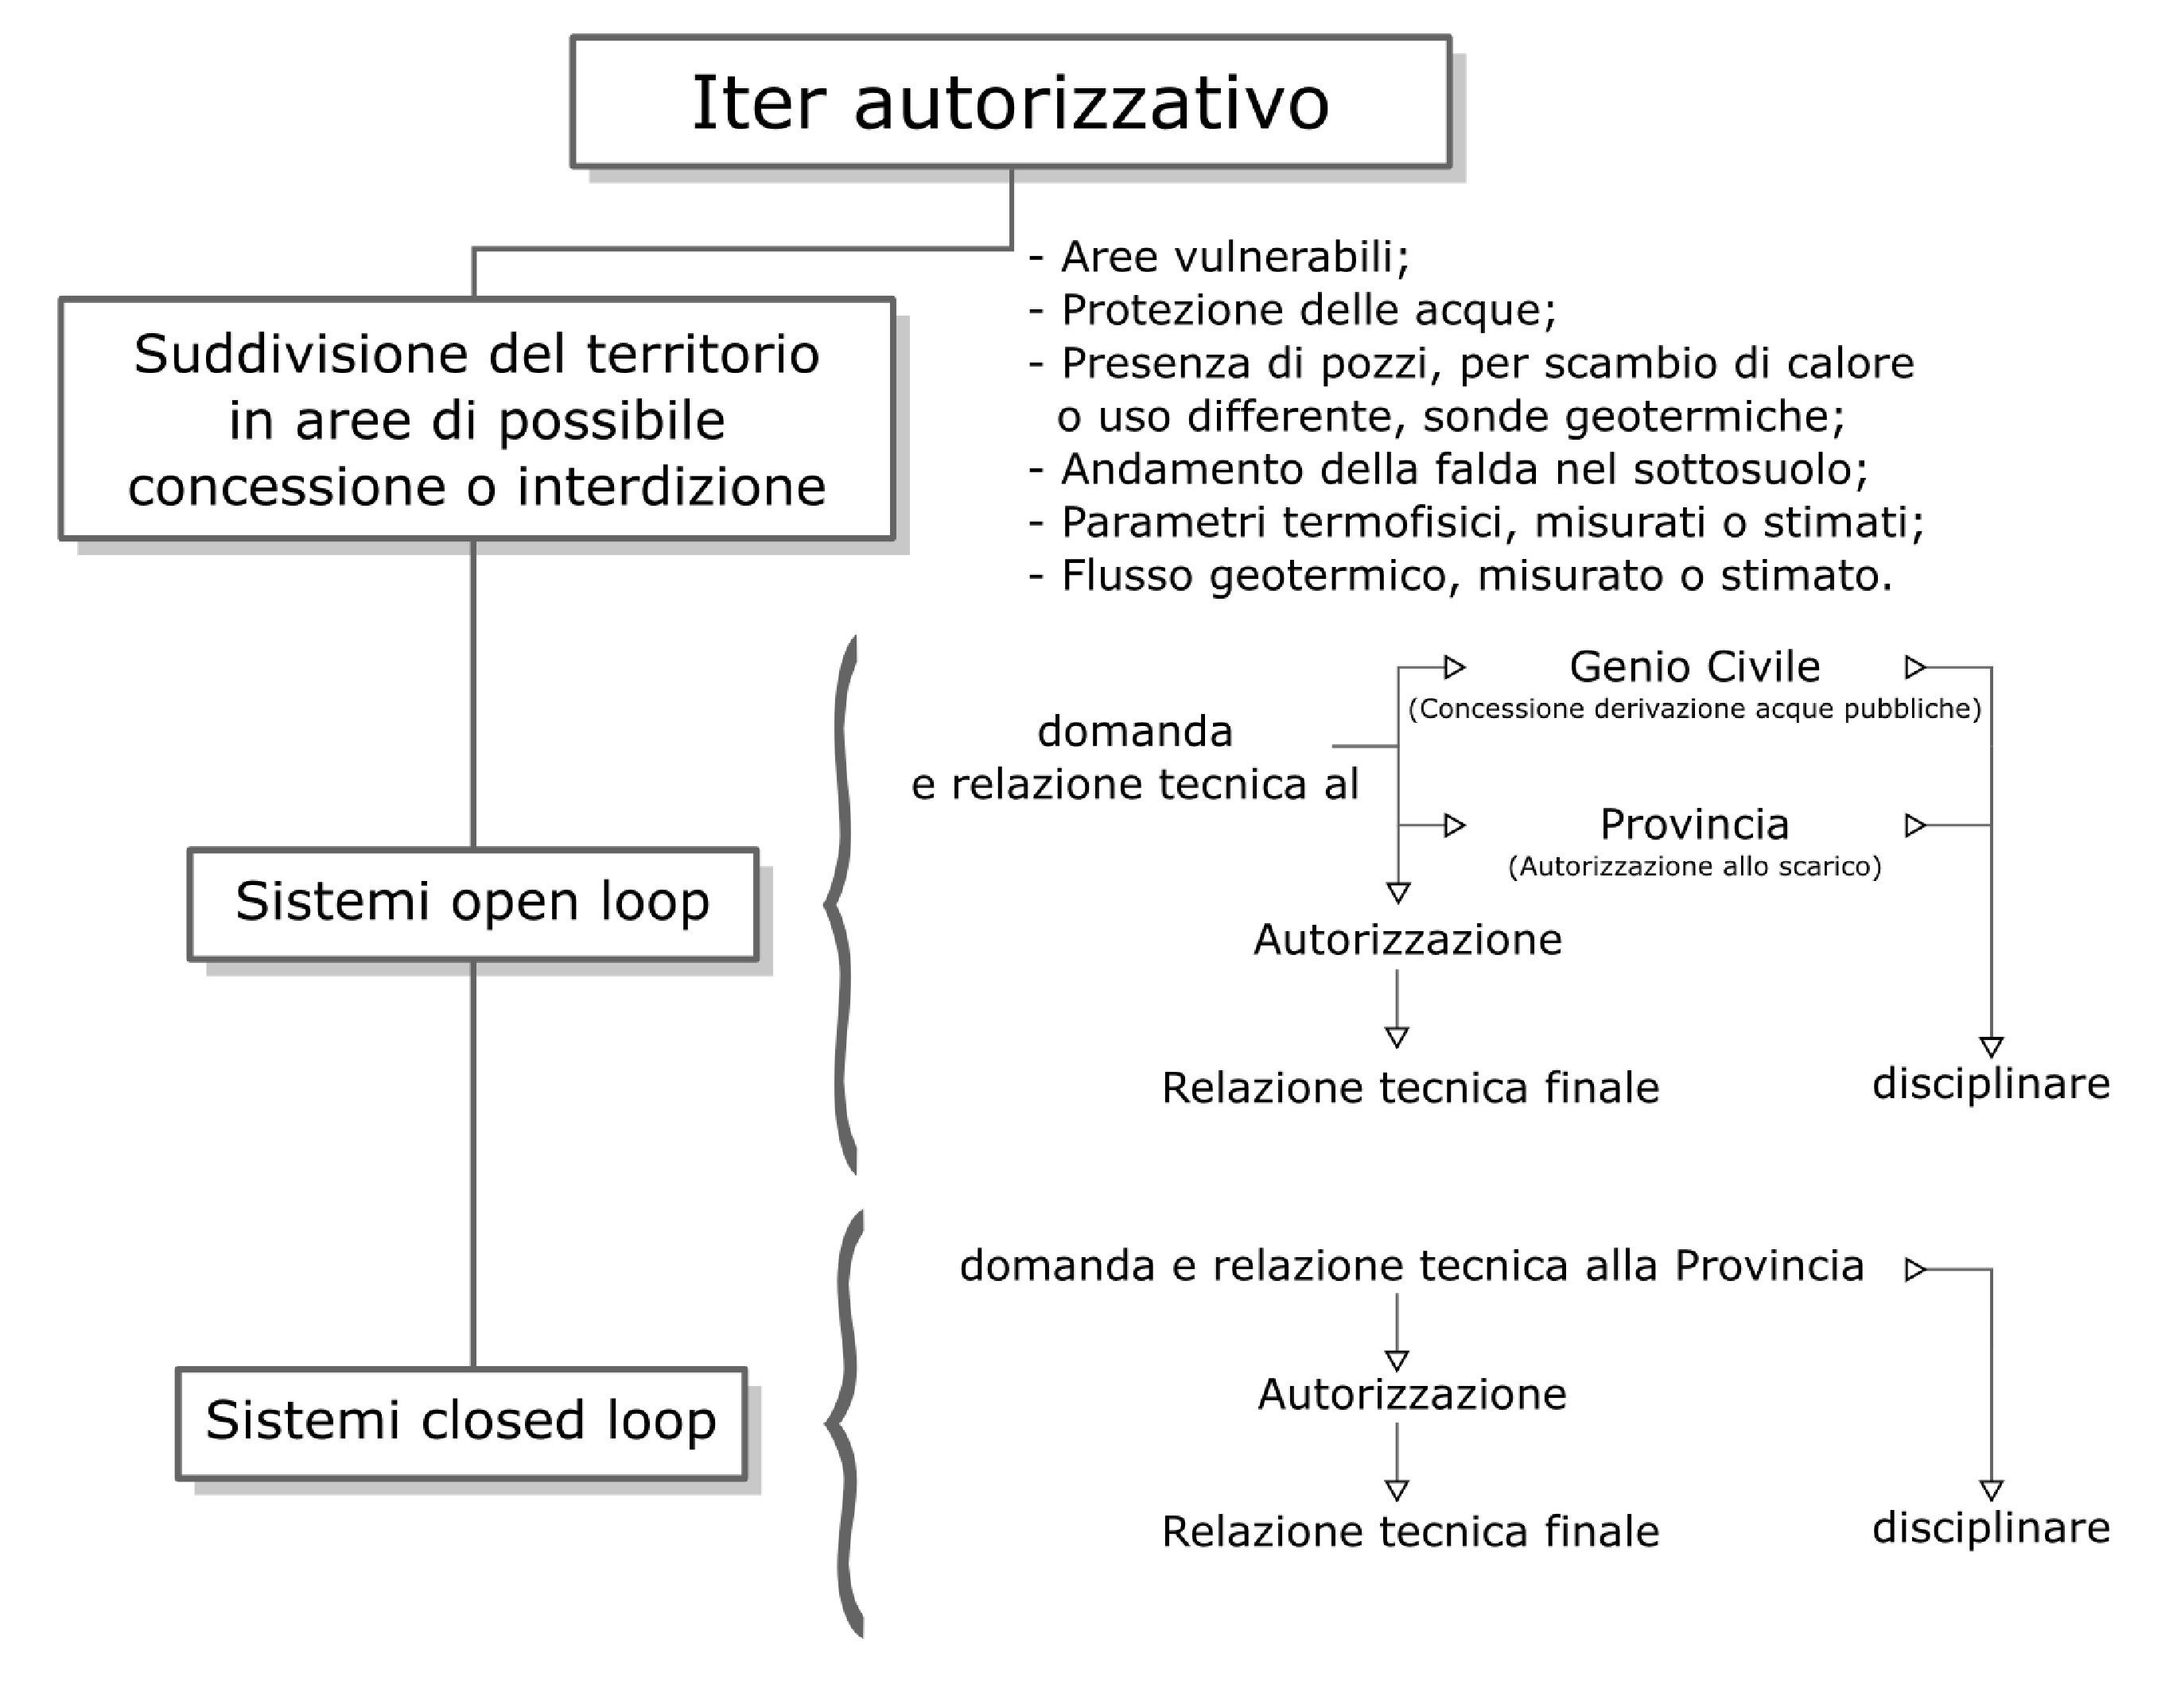
\includegraphics [width=.95\columnwidth, angle=0]{iter_autorizzativo} % height
	\caption{Possibile schema di un iter autorizzativo per i sistemi a circuito aperto e chiuso}
	\label{8fig:iter_autorizzativo}
\end{figure}

\subsection{Pianificazione territoriale}
L'ente di controllo, avvalendosi di una pianificazione del territorio che tenga in considerazione non solo le aree sensibili e di ricarica delle falde, ma anche la presenza di impianti di captazione e geotermici (con la loro impronta idraulica e termica), può autorizzare e inibire l'installazione di nuovi impianti o il loro eventuale ampliamento. Allo scopo sono stati riportati ed elencati software di modellazione numerica delle falde (sottoparagrafo vref{3subsec:modellazionefalde}) e dei campi sonde (paragrafo vref{4sec:grandiimpianti}), che possono essere di aiuto non solo nella progettazione ma anche nelle gestione dinamica e del sottosuolo su piccola e media scala.

Tutto questo lavoro di programmazione e progettazione territoriale può sembrare oneroso e superfluo, per una tecnologia che allo stato attuale è ancora sconosciuta in Italia, ma può rappresentare una soluzione obbligata per l'abbattimento dei costi per la climatizzazione degli edifici e delle emissioni di CO\ped{2} nei prossimi anni. Una autorizzazione limitata alla sola protezione della risorsa idrica nel sottosuolo, può portare alla saturazione e alla sovrapposizione di serbatoi geotermici, se la tecnologia dovesse diventare popolare in tempi brevi e sostituire l'impiantistica tradizionale.

\subsection{Disciplinare}
Una volta concessa l'autorizzazione per l'installazione dell'impianto, l'ente di controllo, nell'usuale disciplinare che regola le clausole e le condizioni d'uso della risorsa, dovrebbe stabilire inoltre la quantità di calore da derivare (media e di picco) e la durata della concessione con modalità e termini per il rinnovo.

\section{Competenze del committente}
Realizzare un sistema geotermico è attualmente oneroso e richiede una progettazione specialistica che pochi installatori possono assicurare o certificare. Il costo iniziale poi è più elevato degli impianti tradizionali e richiede la redazione di relazioni tecniche e idrogeologiche che interessano molteplici figure professionali, sia per il dimensionamento dell'impianto, sia per ottenere la concessione.

\'E bene esserne consapevoli e ricorrere a questo tipo di soluzione per impianti di una certa importanza e che possano servire più utenze. In questo modo si possono ridurre i costi ottimizzando le perforazioni e la gestione del sottosuolo e si possono prevedere analisi e progettazioni più dettagliate.

Inoltre un dimensionamento ottimale dei fabbisogni termici può contribuire a ridurre gli interventi sul terreno che rappresentano la parte più significativa del costo dell'impianto. Vale la pena poi considerare nell'analisi costi/benefici, l'installazione di un sistema ibrido per coprire il carico di picco, se quest'ultimo si raggiunge per poche ore all'anno e far coprire al sistema geotermico il restante \numprint[\%]{90} dell'energia termica richiesta.

Seguendo ed integrando quanto proposto da \cite{anipa}, la committenza per ottenere l'autorizzazione alla realizzazione degli impianti geotermici, dovrà produrre una:
\begin{itemize}
\item domanda da presentare agli organi competenti;
\item relazione idrogeologica preliminare;
%\item competenza della direzione lavori;
\item relazione idrogeologica finale.
\end{itemize}

Di seguito verranno schematizzati i contenuti base di queste domande e relazioni, suddividendole per tipo di impianto ed elencando le competenze della direzione lavori. Ovviamente gli enti di controllo richiederanno maggiori richieste, prescrizioni ed integrazioni a quanto sommariamente elencato. Qui si vuole solo fornire un quadro sintetico e generale, con evidenziate le richieste utili per richiedere ed agevolare l'autorizzazione.

\newpage
\section{Domanda e relazione tecnica preliminare}
La domanda per i due sistemi comprenderà:
\begin{itemize}
\item dati anagrafici del richiedente;
\item dati del progettista e della Direzione Lavori (se differente);
\item dati indicativi della ditta e/o ditte (con eventuali certificazioni);
\item dati significativi dell'impianto (perforazione e installazione);
\item dati indicativi sull'ubicazione dell'impianto.
\end{itemize}

Dovranno poi essere allegati:
\begin{itemize}
\item relazione tecnica di progetto;
\item corografia ubicativa 1:\numprint[]{25000} e planimetria catastale 1:\numprint[]{2000}; 
\end{itemize}

\begin{table}[h]%\footnotesize
	\caption{Requisiti dell'acqua estratta per gli impianti open loop \citep{uni_15450}}
	\label{2tab:valori_richiesti_pdc}
	\centering
	\rowcolors{2}{gray!25}{}
%	\resizebox{0.95\columnwidth}{!}{%
	\begin{tabular}{>{\bfseries}lcc}
	\toprule
componenti		&	valore 		&	unità di misura 	\\
	\midrule
materiale organico	(possibilità di sedimentazione)	&	nessuna		&	-	\\
valore di pH		&	$6,5 \div 9$		&	-	\\
conduttività elettrica		&	$50 \div \numprint[]{1000}$		&	$ \mu \: \mathrm{S} \: \mathrm{cm^{-1}}$	\\
cloruro		&	$< 300$		&	$\mathrm{mg} \: \mathrm{\ell^{-1}}$	\\
ferro e manganese		&	$<1$		&	$\mathrm{mg} \: \mathrm{\ell^{-1}}$	\\
solfato		&	$<2$		&	$\mathrm{mg} \: \mathrm{\ell^{-1}}$ \\
contenuto di O\ped{2}		&	$<2$		&	$\mathrm{mg} \: \mathrm{\ell^{-1}}$	\\
cloro		&	$0\div5$		&	$\mathrm{mg} \: \mathrm{\ell^{-1}}$	\\
nitrato		&	$0\div100$	&	$\mathrm{mg} \: \mathrm{\ell^{-1}}$	\\
	\bottomrule
	\end{tabular}%}
\end{table}

\subsection{Per sistemi open loop}
La relazione tecnica comprenderà:
\begin{description}
\item[$\blacktriangleright$] Dati tecnici
\begin{itemize}
\item potenza dell'impianto ($\mathrm{kW\ped{t}}$);
\item fabbisogno termico mensile, con carico medio e di picco;
\item portata necessaria ($\mathrm{m\ap{3}s\ap{-1}}$);
\item $\Delta \mathrm{T}$ (K o $\celsius$);
\item dotazioni di sicurezza e controllo.
\end{itemize}
\item[$\blacktriangleright$] Dati idrogeologici
\begin{itemize}
\item controllo dei vincoli esistenti nell'area di indagine;
\item inquadramento geologico;
\item idrogeologia del sottosuolo (caratteristiche dell'acquifero, permeabilità e direzione di flusso);
\item censimento dei pozzi esistenti nell'area e di altre perforazioni:
\item analisi qualitativa dell'acqua prelevata e restituita alla falda.
\end{itemize}
\item[$\blacktriangleright$] Progetto
\begin{itemize}
\item schema di progetto per la costruzione dei pozzi, con particolare riferimento a diametri e materiali di filtri e rivestimento;
\item descrizione sulle metodologie previste per eseguire a regola d'arte la cementazione del foro;
\item valutazioni sulle possibili conseguenze relative al prelievo dell'acqua e sulla reimmissione, indicando il $\Delta T$ previsto a breve e a lungo termine (il massimo ammesso è di \numprint[\tccelsius]{5}) e la compatibilità ambientale dello scarico nel corpo recipiente.
\end{itemize}
\end{description}

\newpage
\subsection{Per sistemi closed loop}
La relazione tecnica comprenderà:
\begin{description}
\item[$\blacktriangleright$] Dati tecnici
\begin{itemize}
\item potenza dell'impianto (kW\ped{t});
\item fabbisogno termico mensile, con carico medio e di picco;
\item fluidi, additivi e anticongelanti che verranno utilizzati;
\item $\Delta \mathrm{T}$ (K o $\celsius$);
\item dotazioni di sicurezza e controllo.
\end{itemize}
\item[$\blacktriangleright$] Dati idrogeologici
\begin{itemize}
\item controllo dei vincoli esistenti nell'area di indagine;
\item inquadramento geologico;
\item idrogeologia del sottosuolo (caratteristiche dell'acquifero o degli acquiferi attraversati, permeabilità e direzione di flusso);
\item censimento dei pozzi esistenti nell'area e di altre perforazioni.
\end{itemize}
\item[$\blacktriangleright$] Progetto
\begin{itemize}
\item schema di progetto per la costruzione della sonda o del campo sonde;
\item indicazioni specifiche sulla metodologia di perforazione e sui relativi diametri;
\item descrizione sulle metodologie previste per eseguire a regola d'arte la cementazione del foro.
\item simulazione degli effetti con definizione del tipo, della localizzazione e della quantità della perturbazione termica, a breve e a lungo termine. 
\end{itemize}
\end{description}

\subsection{Compiti della direzione lavori}
Dovrà verificare la corretta esecuzione della posa in opera e controllare che in fase di perforazione la stratigrafia (i cui campioni dovranno essere lasciati a disposizione delle autorità competenti), sia corrispondente a quella prevista in fase di progetto ed in caso contrario predisporre delle adeguate soluzioni tecniche per mitigare le novità emerse.

Dovrà verificare con particolare attenzione gli aspetti relativi alla cementazione, dovendone certificare poi la tenuta. Inoltre eseguirà a seconda dell'impianto realizzato:
\begin{itemize}
\item prova di verifica a pressione della tenuta;
\item prova di portata nel pozzo di presa e di immissione in quello di scarico.
\end{itemize}

\newpage
\section{Relazione tecnica finale}
\subsection{Per sistemi open loop}
Comprenderà:
\begin{itemize}
\item dati stratigrafici effettivi;
\item schema effettivo dei pozzi realizzati;
\item dati idrogeologici derivanti anche dai risultati delle prove di pompaggio eseguite;
\item valutazioni sulle possibili conseguenze del prelievo e della restituzione;
\item calcolo dell'area influenzata dal $\Delta T$ nel breve e lungo termine (bulbo termico).
\end{itemize}

Verrà allegata:
\begin{itemize}
\item la planimetria con le effettive ubicazioni dei pozzi eseguiti con evidenziato il raggio di influenza del $\Delta T$ a breve e lungo termine.
\end{itemize}

La D.L. attesterà mediante dichiarazione sottoscritta la tenuta della cementazione, dell'impianto, la non interferenza tra le falde eventualmente presenti sia tra loro che con la superficie e la compatibilità ambientale dello scarico nel corpo recipiente.

\subsection{Per sistemi closed loop}
Comprenderà:
\begin{itemize}
\item dati stratigrafici effettivi;
\item schema effettivo dei pozzi realizzati;
\item variazioni rispetto al progetto preliminare;
\item dati relativi alla cementazione eseguita;
\item simulazione effettiva degli effetti con definizione del tipo, della localizzazione e della quantità della perturbazione termica, a breve e a lungo termine.
\end{itemize}

Verrà allegata:
\begin{itemize}
\item la planimetria con le effettive ubicazioni delle sonde eseguite e la perturbazione termica, a breve e a lungo termine.
\end{itemize}

La D.L. attesterà mediante dichiarazione sottoscritta la tenuta della cementazione e dell'impianto e la non interferenza tra le falde eventualmente presenti, sia tra loro che con la superficie.

% APPENDICES
%\appendix
%\include{appendix1/appendix1}
%\include{appendix2/appendix2}

%% BACKMATTER %%
% The pages inside of backmatter are in Arabic numerals and the chapters will not have numeration
\backmatter

% BIBLIOGRAPHY WITH BIBTEX %
%*******************************************************
% Bibliography
%*******************************************************
\cleardoublepage
\phantomsection
\addcontentsline{toc}{chapter}{\bibname}
\nocite{*}
% The style can be: classic, plainnat, abbrvnat or unsrtnat
\bibliographystyle{classic}
\bibliography{bibliography}
%

\vspace{2.5cm}
\begin{Large}Websites consulted\end{Large}
\begin{itemize}
\item A.N.I.P.A, il portale della perforazione	-- \url{www.anipapozzi.it}
\item Edilportale.com, il portale dell'edilizia -- \url{www.edilportale.com}
\item EGEC, European Geothermal Energy Council -- \url{www.egec.org}
\item Geo Heat -- \url{geoheat.oit.edu}
\item Geo Net srl -- \url{www.geo-net.it}
\item IGA, International Geothermal Association -- \url{www.geothermal-energy.org}
\item ScienceDirect -- \url{www.sciencedirect.com}
\item SpringerLink -- \url{www.springerlink.com}
\item Therm-tech Technological Engineering -- \url{www.therm-tech.it}
\item UGI, Unione Geotermica Italiana -- \url{www.unionegeotermica.it}
\item Wikipedia -- \url{www.wikipedia.org}
%\item -- \url{library.isgs.uiuc.edu}
\end{itemize}


% All the sources are described in a file named bibliography.bib
% if you want to cite one in the text:
% \citep{label}
% In order to update the bibliography you have to execute:
% bibtex main (without ".tex")

% INDEX %
\cleardoublepage
% To help hyperref to jump to the correct page
\phantomsection
% To add the Index in the table of contents
\addcontentsline{toc}{chapter}{Indice analitico}
% Prints the Index
\printindex
% To add an item in it, write the \index{WORD} after the word to highlight:
% WORD\index{WORD}
% In order to update the Index you have to execute:
% makeindex main (without ".tex")

% A typical session involving a bibliography, an index and so on would require:
% pdflatex main
% makeindex -s main.ist -t main.alg -o main.acr main.acn
% makeindex -s main.ist -t main.glg -o main.gls main.glo
% bibtex main
% pdflatex main
% pdflatex main
% makeindex main
% makeindex -s main.ist -t main.alg -o main.acr main.acn
% makeindex -s main.ist -t main.glg -o main.gls main.glo
% pdflatex main
% pdflatex main
\end{document}
